\chapter{Clustering}

\section{Auxiliary Graph}
From the clustered graph a weighted auxiliary graph is defined for each frame, denoted as $G^{aux}$ := ($V$, $E^{aux}$, $w^{aux}$). \\
The vertices of this auxiliary graph are the same as in the original graph $G$, but the edge set is comprised of a subset of edges that only connect vertices belonging to different clusters.
The weight of every edge is calculated by applying Euclidean norm (Formula \ref{formula:normalization}) between pairs of vectors.
Edges that do not represent direct physical connections are ignored.
One of these edges in the auxiliary graph will be the edge associated with the origin of motion.
\\

Considering, for example, a graph $G$ with 3 clusters (see Figure \ref{fig:graph_g}), we can visualize which edges will be involved in the auxiliary graph (Figure \ref{fig:aux_graph}).
\begin{figure}[H]
  \begin{subfigure}{0.45\textwidth}
    \centering
    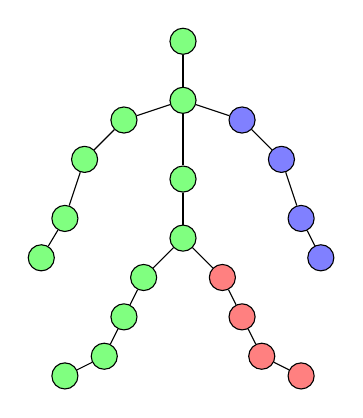
\begin{tikzpicture}
      \node[circle, draw, minimum size=0.1cm] (1) at (3.5,-1.25) [fill=green!50] {};
      \node[circle, draw, minimum size=0.1cm] (2) at (6.5, -1.25) [fill=red!50] {};
      \node[circle, draw, minimum size=0.1cm] (3) at (4,-1) [fill=green!50] {};
      \node[circle, draw, minimum size=0.1cm] (4) at (6, -1) [fill=red!50] {};
      \node[circle, draw, minimum size=0.1cm] (5) at (4.25,-0.5) [fill=green!50] {};
      \node[circle, draw, minimum size=0.1cm] (6) at (5.75,-0.5) [fill=red!50] {};
      \node[circle, draw, minimum size=0.1cm] (7) at (4.5,0) [fill=green!50] {};
      \node[circle, draw, minimum size=0.1cm] (8) at (5, 0.5) [fill=green!50] {};
      \node[circle, draw, minimum size=0.1cm] (9) at (5.5,0) [fill=red!50] {};
      \node[circle, draw, minimum size=0.1cm] (10) at (5,1.25) [fill=green!50] {};
      \node[circle, draw, minimum size=0.1cm] (11) at (3.2, 0.25) [fill=green!50] {};
      \node[circle, draw, minimum size=0.1cm] (12) at (6.75,0.25) [fill=blue!50] {};
      \node[circle, draw, minimum size=0.1cm] (13) at (3.5, 0.75) [fill=green!50] {};
      \node[circle, draw, minimum size=0.1cm] (14) at (6.5, 0.75) [fill=blue!50] {};
      \node[circle, draw, minimum size=0.1cm] (15) at (3.75,1.5) [fill=green!50] {};
      \node[circle, draw, minimum size=0.1cm] (16) at (6.25,1.5) [fill=blue!50] {};
      \node[circle, draw, minimum size=0.1cm] (17) at (4.25,2) [fill=green!50] {};
      \node[circle, draw, minimum size=0.1cm] (18) at (5,2.25) [fill=green!50] {};
      \node[circle, draw, minimum size=0.1cm] (19) at (5.75,2) [fill=blue!50] {};
      \node[circle, draw, minimum size=0.1cm] (20) at (5,3) [fill=green!50] {};  
      \foreach \source/\dest/\label/\xshiftval in {20/18//0, 18/17//0, 18/19//0, 17/15//0, 15/13//0, 13/11//0, 19/16//0, 16/14//0, 14/12//0, 18/10//0, 10/8//0, 8/7//0, 7/5//0, 5/3//0, 3/1//0, 8/9//0, 9/6//0, 6/4//0, 4/2//0}
        \path (\source) edge node[xshift=\xshiftval] {\label} (\dest);
    \end{tikzpicture}
    \caption{Graph $G$}
    \label{fig:graph_g}
  \end{subfigure}
  \hspace{0.01\linewidth}
  \begin{subfigure}{0.45\linewidth}
    \centering
    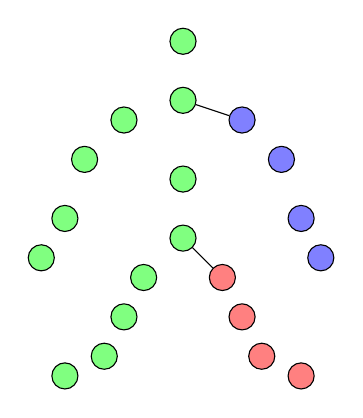
\begin{tikzpicture}
      \node[circle, draw, minimum size=0.1cm] (1) at (3.5,-1.25) [fill=green!50] {};
      \node[circle, draw, minimum size=0.1cm] (2) at (6.5, -1.25) [fill=red!50] {};
      \node[circle, draw, minimum size=0.1cm] (3) at (4,-1) [fill=green!50] {};
      \node[circle, draw, minimum size=0.1cm] (4) at (6, -1) [fill=red!50] {};
      \node[circle, draw, minimum size=0.1cm] (5) at (4.25,-0.5) [fill=green!50] {};
      \node[circle, draw, minimum size=0.1cm] (6) at (5.75,-0.5) [fill=red!50] {};
      \node[circle, draw, minimum size=0.1cm] (7) at (4.5,0) [fill=green!50] {};
      \node[circle, draw, minimum size=0.1cm] (8) at (5, 0.5) [fill=green!50] {};
      \node[circle, draw, minimum size=0.1cm] (9) at (5.5,0) [fill=red!50] {};
      \node[circle, draw, minimum size=0.1cm] (10) at (5,1.25) [fill=green!50] {};
      \node[circle, draw, minimum size=0.1cm] (11) at (3.2, 0.25) [fill=green!50] {};
      \node[circle, draw, minimum size=0.1cm] (12) at (6.75,0.25) [fill=blue!50] {};
      \node[circle, draw, minimum size=0.1cm] (13) at (3.5, 0.75) [fill=green!50] {};
      \node[circle, draw, minimum size=0.1cm] (14) at (6.5, 0.75) [fill=blue!50] {};
      \node[circle, draw, minimum size=0.1cm] (15) at (3.75,1.5) [fill=green!50] {};
      \node[circle, draw, minimum size=0.1cm] (16) at (6.25,1.5) [fill=blue!50] {};
      \node[circle, draw, minimum size=0.1cm] (17) at (4.25,2) [fill=green!50] {};
      \node[circle, draw, minimum size=0.1cm] (18) at (5,2.25) [fill=green!50] {};
      \node[circle, draw, minimum size=0.1cm] (19) at (5.75,2) [fill=blue!50] {};
      \node[circle, draw, minimum size=0.1cm] (20) at (5,3) [fill=green!50] {};  
      \foreach \source/\dest/\label/\xshiftval in {18/19//0, 8/9//0}
        \path (\source) edge node[xshift=\xshiftval] {\label} (\dest);
    \end{tikzpicture}
    \caption{Auxiliary graph $G^{aux}$}
    \label{fig:aux_graph}
  \end{subfigure}
\end{figure}


\section{Weighted Degree Centrality}
To identify the edge involved in the OoM, we use the WDC, as explained in Section \ref{subsec:weighted_degree}.
For each frame, we keep track of the two nodes with the highest WDC.
At the end of this process, among the selected nodes, we will choose the two nodes that have been chosen as the highest most frequently.
At this stage, we will examine in the $G^{aux}$ to which edges belonging to $E^{aux}$ these two winning nodes are connected, and these two edges will be considered as the predicted OoM.

\section{Results}
The OoM was classified using three distinct features: speed, acceleration and angular momentum, as described in Section \ref{sec:features}.
For each feature, we calculated the accuracy of the method in predicting the correct edge compared to the true label.\\
In Table \ref{tab:clust_results} we can see the results.


\begin{table}[H]
  \centering
  \begin{tabular}{||>{\centering\arraybackslash}p{1.2cm}||>{\centering\arraybackslash}p{4.3cm}||>{\centering\arraybackslash}p{4.3cm}||>{\centering\arraybackslash}p{4.3cm}||}
  \hline
  & \textbf{Speed} & \textbf{Acceleration} & \textbf{Angular Momentum} \\
  \hline
  \textbf{WDG} & 28.3\%  & 26.7\%  & 36.6\%  \\
  \hline
  \end{tabular}
  \caption{Classification accuracy with WDC on the overall dataset}
  \label{tab:clust_results}
\end{table}

Even though these results are not impressive, they are still better than a random approach, where two random nodes are selected, and by examining which edges in the auxiliary graph they are connected to, they are compared to the ground truth. \\
Such an approach, in fact, achieves an accuracy of 19\%.
Figure \ref{fig:wdc_results} shows the distribution of the results for each edge of the dataset:
\begin{figure}
  \centering
  \includegraphics[width=0.85\textwidth]{wdc_results.png}
  \caption{Joints and frequency of the dataset and the correctly classified WDC algorithm}
  \label{fig:wdc_results}
\end{figure}